
This chapter discusses Motzkin, Schröder, and Łukasiewicz paths, combinatorial objects that will be generated by the algorithm in Chapter \ref{chap:luka-graycode}.
Motzkin, Schröder, and Łukasiewicz paths all provide generalizations of Dyck paths.  
All three languages retain the requirement that the path start at the origin, end on the $x$ axis, and never step below the $x$ axis.  However, the three languages vary from Dyck paths in the types of steps they allow.  Section \ref{sec:motzkin} will discuss Motzkin paths, Section \ref{sec:schroder} Schröder paths, and Section \ref{sec:lukasiewicz} will discuss Łukasiewicz paths.

\section{Motzkin Paths}\label{sec:motzkin}
Recall the interpretation of Dyck words as paths in the Cartesian plane from Section \ref{sec:Dycks}.
Motzkin paths use (1,0) horizontal steps in addition to $(1,1)$ and $(1,-1)$ steps. 
% The number of Motzkin and Schröder paths termminating at $(n,0)$ are counted by the $n\thh$ Motzkin and Schröder numbers respectively.  These sequences are illustrated below for $n \ge 0$ along with their respective entries in the Online Encyclopedia of Integer Sequences (OEIS) \cite{oeis}.
The number of Motzkin paths termminating at $(n,0)$ is counted by the $n\thh$ Motzkin number.  This sequence is illustrated below for $n \ge 0$ along with its corresponding OEIS entry.


\begin{align}
\mathcal{M}_n &= 1, 1, 2, 4, 9, 21, 51, \ldots  & \text{OEIS} \text{A}001006
\end{align}

The Motzkin numbers are named for $20\thh$ century Israeli-American mathematician Theodore Motzkin and are closely related to the Catalan numbers.  In particular, the Motzkin numbers can be expressed in terms of binomial coefficients and Catalan numbers via the following equation:

\begin{equation}
	\M_n = \sum_{k=0}^{\lfloor n/2 \rfloor} {n \choose 2k}\C_k
\end{equation}

And inversely, 

\begin{equation}
	\C_{n+1} = \sum_{k=0}^{n} {n \choose k}\M_k
\end{equation}

The Motzkin numbers have many additional combinatorial interpretations, which are often similar to combinatorial interpretations of the Catalan numbers.  For example, $\C_n$ counts the number of ordered trees with $n+1$ nodes, while $\M_n$ counts the number of ordered trees with $n+2$ nodes with the restriction that no node except for the root has exactly one child (although the root need not have exactly one child). Donaghey and Shapiro's \emph{Motzkin Numbers} demonstrates this as well as many other interesting bijections \cite{donaghey1977motzkin}.

\section{Schröder Paths}\label{sec:schroder}

Schröder paths are identical to Motzkin paths except they allow for $(2,0)$ horizontal steps instead of $(1,0)$.  The number of Schröder paths terminating at $(2n,0)$ is counted by the $n\thh$ big Schröder number.  This sequence is illustrated below for $n \ge 0$ along with its corresponding OEIS entry.

\begin{align}
\mathcal{S}_n &= 1, 2, 6, 22, 90, 394, 1806, \ldots & \text{OEIS} \text{A}006318
\end{align}

The use of $(2,0)$ horizontal steps seems arbitrary at first but has a number of useful properties.  For example, unlike Motzkin paths, Schröder paths retain the property of Dyck paths that each path must terminate at $(2n,0)$ for some integer $n$.  Conversely, one-length horizontal step in Motzkin words allows Motzkin paths to termminate at odd positions on the $x$ axis.  

The big Schröder numbers are named for $19\thh$ century German mathematician Ernst Schröder.  They are related to but distinct from the little Schröder numbers, which have the fascinating history of potentially being discovered thousands of years before the Catalan, Motzkin, and big Schröder numbers by the Greek astronomer Hipparchus.  See \cite{stanley1997hipparchus} for a brief history of this discovery and \cite{bobzien2011combinatorics} for an in-depth reconstruction of Hipparchus's logic. 

Another combinatorial interpretation of the big Schröder numbers is the number of rectangular partitions constrained to lie on $n+1$ points \cite{ackerman2004number}.  Shapiro and Sulanke's \emph{Bijections for the Schröder Numbers} gives many other related interpretations of the Schröder numbers \cite{shapiro2000bijections}.

We encode both Motzkin and Schröder paths with southeast steps encoded as zeroes, horizontal steps as ones, and northeast steps as twos.
Consequently, in the context of fixed-content generation, Motzkin and Schröder paths are identical.  However, their Cartesian plane representations will differ in the length of horizontal steps. As a basic example, the Motzkin/Schröder word $2,1,1,0$ terminates at the point $(4,0)$ if interpreted as a Motzkin path and $(6,0)$ if interpreted as a Schröder path.  We refer to these integer based encodings as \emph{Motzkin words} or \emph{Schröder words}.  Motzkin and Schröder words have the property that each prefix of the word has a sum at least as large as its length, and the whole word has a sum equal to its length.



\section{Łukasiewicz Paths}\label{sec:lukasiewicz}

Łukasiewicz paths allow $(1,-1)$ steps, $(1,0)$ steps and any $(1,k)$ step where $k$ is a positive integer. We encode each $(1,k)$ step in a Łukasiewicz path as $k+1$ and therefore encode an Łukasiewicz path of length $n$ as a sequence of integers.  We call the resulting string of integers a \emph{Łukasiewicz word}.  Like Motzkin and Schröder words, Łukasiewicz words have the property that the sum of each prefix of a Łukasiewicz word is at least as great as the prefix's length and the sum of an entire Łukasiewicz word is equal to its length.. 

The number of Łukasiewicz paths terminating at $(n,0)$ is counted by the $n\thh$ Catalan number, $\C_n$. Łukasiewicz paths are therefore in bijective correspondence with the Catalan objects discussed in in Chapter \ref{chap:catalan}, sharing a particularly nice correspondence with ordered trees. In particular, a Łukasiewicz word of length $n$ can be constructed from an ordered tree with $n+1$ nodes via a preorder listing each ordered tree node's number of children, excluding the final leaf.  See Figure \ref{fig:lukatrees} for an illustration of this bijection.
Our algorithm in Chapter $\ref{chap:luka-graycode}$ will generate Łukasiewicz words with \emph{fixed content}.

% These paths can be encoded in a number of different ways.  In a \emph{-1-based encoding}, each $(1,i)$ step is encoded as i, and every prefix must have a nonnegative sum.  In a \emph{0-based encoding}, each $(1,i)$ step is encoded as $i+1$, and the sum of every prefix must be as large as its length. We primarily use the 0-based encoding. See Fig. \ref{fig:paths}  for examples of these paths using the 0-based encoding. 

\begin{figure}[]
	\centering
	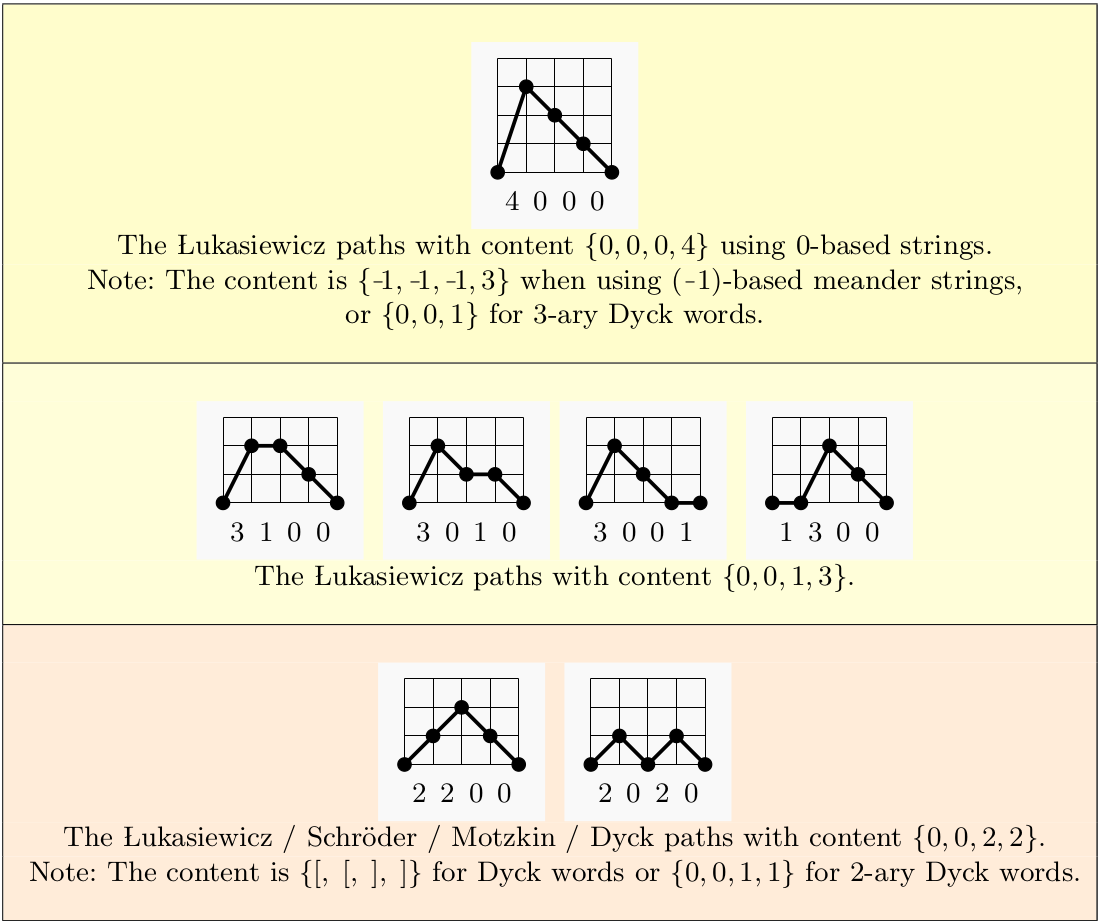
\includegraphics[width = .95 \textwidth]{paths.png}
	\caption{Łukasiewicz, Motzkin, and Schröder words and paths termminating at $(4,0)$.}
	\label{fig:paths}
\end{figure}


% The number of Dyck words with n zeroes and n ones are counted by the $n$st Catalan number.  Similarly, the number of Motzkin and Schröder paths of order $n$ are counted by the $n\thh$ Motzkin and big Schröder number respectively. The number of Łukasiewicz paths of order $n$ are counted by the $n-1$st Catalan number. 
% Motzkin, Schröder, and Łukasiewicz paths bear a number of interesting bijective correspondences with other combinatorial objects. Richard Stanely's \emph{Catalan Objects} outlines hundreds of interesting examples.  

% Łukasiewicz paths  of order $n$ bear a particularly nice correspondence to rooted ordered trees with $n$ nodes. See Fig. \ref{fig:lukatrees} for an illustration of this.

\begin{figure}[]
	\centering
	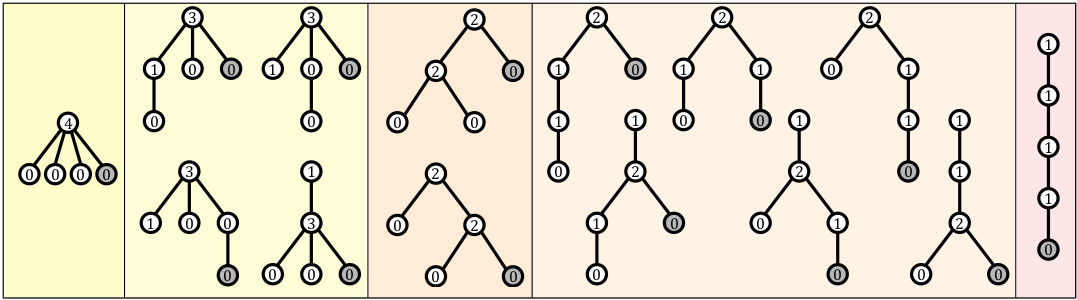
\includegraphics[width = .95 \textwidth]{trees.png}
	\caption[The $\mathcal{C}_4$=14 Łukasiewicz paths of order $n=4$ are in bijective correspondence with the 14 rooted ordered trees with $n+1=5$ nodes.]{The $\mathcal{C}_4$=14 Łukasiewicz paths of order $n=4$ are in bijective correspondence with the 14 rooted ordered trees with $n+1=5$ nodes.  Ordered tree nodes are labelled by their number of children.  Given a tree, a Łukasiewicz word is obtained by recording the number of children of each node in preorder traversal; the zero from the rightmost leaf is omitted.  For example, the two trees in the middle section correspond to 2200 (top) and 2020 (bottom) respectively.}
	\label{fig:lukatrees}
\end{figure}

% TODO: bijections, mirror chapter 2

